\section{Introduction}

what is the need for resilience\\

what are the challenges we face with resilience in a deferred execution model, with all the decisions taken at runtime via a mapper ? \\

what are the advantages that we derive from the same ?\\
The needle in the resilience spectrum can be much finer than ABFT, sub-tree DAG based, snapshot based, relocatable-finish based, strategies. Dynamic and deferred being the key.

what are the advantages that we derive from having multiple wavefront ?\\
how do we ensure minimal overhead ?\\

Is it really a resilience framework, or a glorified garbage collector ?\\


how is it different from x10, parsec, charm++\\
	- they also allow tasks to be marked as resilience\\
	- x10 allows finish blocks, exception semantics.\\
	- what are the exception semantics that we are providing\\


what about regent ? where do we stand there ?\\

what about local vs global recovery\\
	- can we recover from a node failure\\
	- can we recover from an exception, what are the semantics that we provide here\\
	- can we recover from ECC errors, \\
	- can we fix these errors ?\\
	- can we recover from I/O errors ?\\ 
	- can we recover from non-SingleTasks, what is recovery for index space tasks, must epoch tasks\\

what is the memory consistency model ? what is the state of the regions, the tasks that are physically dependent but are not logically dependent ?\\
	

experiments: circuit, miniAero, Soleil-X, stencil, (S3D ?)\\

\begin{figure}
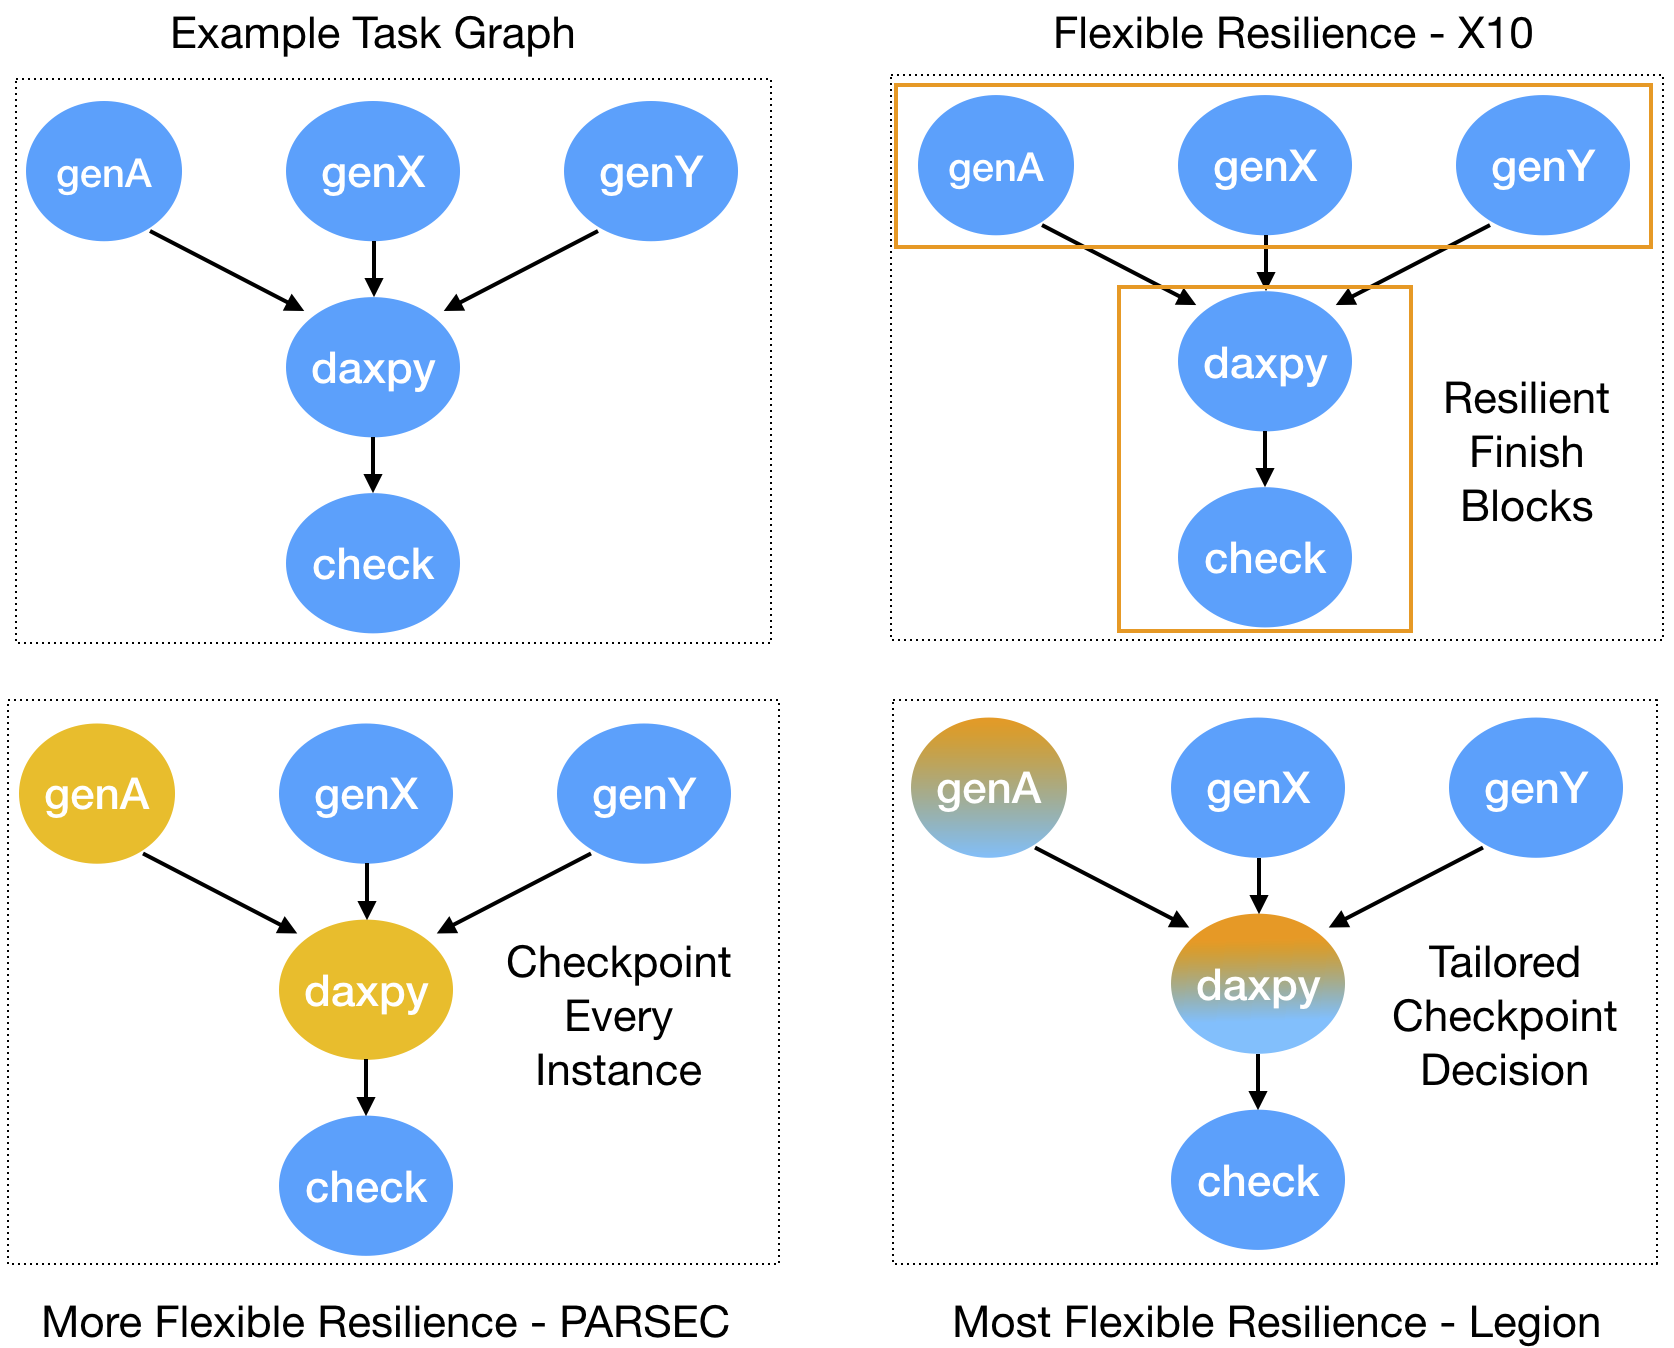
\includegraphics[width=.45\textwidth]{images/spectrum_x10_parsec_legion_policies.png}
\caption{A spectrum of resilience policies supported by different state-of-the-art parallel runtimes.}
\end{figure}
